\let\negmedspace\undefined
\let\negthickspace\undefined
\documentclass[journal,12pt,twocolumn]{IEEEtran}

\usepackage{cite}
\usepackage{amsmath,amssymb,amsfonts,amsthm}
\usepackage{algorithmic}
\usepackage{graphicx}
\usepackage{textcomp}
\usepackage{xcolor}
\usepackage{txfonts}
\usepackage{listings}
\usepackage{enumitem}
\usepackage{mathtools}
\usepackage{gensymb}
\usepackage[breaklinks=true]{hyperref}
\usepackage{tkz-euclide} % loads  TikZ and tkz-base
\usepackage{listings}
\usepackage{circuitikz}
\usepackage{graphicx}

%\newcounter{MYtempeqncnt}
\DeclareMathOperator*{\Res}{Res}
%\renewcommand{\baselinestretch}{2}
\renewcommand\thesection{\arabic{section}}
\renewcommand\thesubsection{\thesection.\arabic{subsection}}
\renewcommand\thesubsubsection{\thesubsection.\arabic{subsubsection}}

\renewcommand\thesectiondis{\arabic{section}}
\renewcommand\thesubsectiondis{\thesectiondis.\arabic{subsection}}
\renewcommand\thesubsubsectiondis{\thesubsectiondis.\arabic{subsubsection}}

% correct bad hyphenation here
\hyphenation{op-tical net-works semi-conduc-tor}
\def\inputGnumericTable{}                                 %%

\lstset{
	frame=single,
	breaklines=true,
	columns=fullflexible
}

\newtheorem{theorem}{Theorem}[section]
\newtheorem{problem}{Problem}
\newtheorem{proposition}{Proposition}[section]
\newtheorem{lemma}{Lemma}[section]
\newtheorem{corollary}[theorem]{Corollary}
\newtheorem{example}{Example}[section]
\newtheorem{definition}[problem]{Definition}
\newcommand{\BEQA}{\begin{eqnarray}}
	\newcommand{\EEQA}{\end{eqnarray}}
\newcommand{\define}{\stackrel{\triangle}{=}}
\newcommand\figref{Fig.~\ref}
\newcommand\tabref{Table~\ref}
\bibliographystyle{IEEEtran}
%\bibliographystyle{ieeetr}


\providecommand{\mbf}{\mathbf}
\providecommand{\pr}[1]{\ensuremath{\Pr\left(#1\right)}}
\providecommand{\qfunc}[1]{\ensuremath{Q\left(#1\right)}}
\providecommand{\sbrak}[1]{\ensuremath{{}\left[#1\right]}}
\providecommand{\lsbrak}[1]{\ensuremath{{}\left[#1\right.}}
\providecommand{\rsbrak}[1]{\ensuremath{{}\left.#1\right]}}
\providecommand{\brak}[1]{\ensuremath{\left(#1\right)}}
\providecommand{\lbrak}[1]{\ensuremath{\left(#1\right.}}
\providecommand{\rbrak}[1]{\ensuremath{\left.#1\right)}}
\providecommand{\cbrak}[1]{\ensuremath{\left\{#1\right\}}}
\providecommand{\lcbrak}[1]{\ensuremath{\left\{#1\right.}}
\providecommand{\rcbrak}[1]{\ensuremath{\left.#1\right\}}}
\theoremstyle{remark}
\newtheorem{rem}{Remark}
\newcommand{\sgn}{\mathop{\mathrm{sgn}}}
\providecommand{\abs}[1]{\left\vert#1\right\vert}
\providecommand{\res}[1]{\Res\displaylimits_{#1}}
\providecommand{\norm}[1]{\left\lVert#1\right\rVert}
%\providecommand{\norm}[1]{\lVert#1\rVert}
\providecommand{\mtx}[1]{\mathbf{#1}}
\providecommand{\mean}[1]{E\left[ #1 \right]}
\providecommand{\fourier}{\overset{\mathcal{F}}{ \rightleftharpoons}}
%\providecommand{\hilbert}{\overset{\mathcal{H}}{ \rightleftharpoons}}
\providecommand{\system}{\overset{\mathcal{H}}{ \longleftrightarrow}}
%\newcommand{\solution}[2]{\textbf{Solution:}{#1}}
\newcommand{\solution}{\noindent \textbf{Solution: }}
\newcommand{\cosec}{\,\text{cosec}\,}
\providecommand{\dec}[2]{\ensuremath{\overset{#1}{\underset{#2}{\gtrless}}}}
\newcommand{\myvec}[1]{\ensuremath{\begin{pmatrix}#1\end{pmatrix}}}
\newcommand{\mydet}[1]{\ensuremath{\begin{vmatrix}#1\end{vmatrix}}}
\renewcommand{\abstractname}{Question}

\let\vec\mathbf

\vspace{3cm}


\newcommand{\permcomb}[4][0mu]{{{}^{#3}\mkern#1#2_{#4}}}
\newcommand{\comb}[1][-1mu]{\permcomb[#1]{C}}

%\IEEEpeerreviewmaketitle

\newcommand \tab [1][1cm]{\hspace*{#1}}
%\newcommand{\Var}{$\sigma ^2$}
\usepackage{amssymb}
\usepackage{amsmath}
\title{
	
	\title{NCERT Maths 11.9.2 Q6}
	\author{EE23BTECH11212 - MANUGUNTA MEGHANA SAI$^{*}$% <-this % stops a space
	}
	
	
}
\begin{document}
	
	\maketitle
	
	\textbf{Question:} 
	If the sum of certain number of terms in a AP 25,22,19,... is 116. Find the last term.\\
	\\

	\solution
	 \begin{table}[h!]
	 	\centering
	 	\resizebox{6cm}{!}{
	 		\begin{tabular}{|c|c|c|}
	\hline
	\textbf{Symbol} & \textbf{Value} &
	\textbf{Description}\\[6pt]
	\hline
	L &  $80m\,
	\text{H}$ & Inductance\\[6pt]
	\hline 
	C &  $60\, \mu\text{F}$ & Capacitance \\[6pt]
	\hline
	R &  $15\, \Omega$ & Resistance\\[6pt]
	\hline
	V & $230\, \text{V}$ & Voltage\\[6pt]
	\hline
	f & $50\, \text{Hz}$ & Frequency\\[6pt]
	\hline
\end{tabular}
	 	}
	 	\caption{Given Parameters}
	 	\label{tab:my_label}
	 \end{table}

	\begin{align}
		x(n) = (25 - 3n)u(n)
		\label{eq:1}
	\end{align}
     Applying Z transform:
     \begin{align}
     	x(z) &=\frac{25}{1-z^{-1}} - \frac{3z^{-1}}{(1-z^{-1})^2}\\
     	&= \frac{25-28z^{-1}}{(1-z^{-1})^2} 
     \end{align}
     Region of Convergence or R.O.C :
     \begin{align}
     	\abs{z}>1
     \end{align}
For AP, the sum of first n+1 terms can be written as :
\begin{align}
	 y(n)&=x(n)*u(n)
\end{align}  
Applying Z transform on both sides
\begin{align}
	Y(z) &= x(z)u(z)\\
	&=\frac{25}{(1-z^{-1})^2} - \frac{3z^{-1}}{(1-z^{-1})^3}
\end{align}
Using contour integration to find inverse Z transform:
\begin{align}
	Y(n) &= \frac{1}{2\pi j} \oint_C Y(z) z^{n-1} dz\\
	&= \frac{1}{2\pi j} \oint_C [\frac{25}{(1-z^{-1})^2} - \frac{3z^{-1}}{(1-z^{-1})^3} ]z^{n-1} dz
\end{align}
The sum of the terms of the sequence is computed using the residue theorem, expressed as $R_i$, which represents the residue of the Z-transform at $ z=1 $ for the expression $ Y(z) $.
\begin{align}
	R_i=R_1 + R_2
\end{align}
 $R_1$ and $R_2$ are residues calculated at the poles of the Z-transform.
\begin{align}
		R_1 &= \frac{1}{{(2-1)!}} \left. \frac{d (25z^{n+1})}{dz} \right|_{z=1} \\
	&=25(n+1)
\end{align}
\begin{align}
	R_2 &= \frac{1}{{(3-1)!}} \left. \frac{d^2(-3z^{n+1})}{dz^2} \right|_{z=1} \\
	&= \frac{-3}{2}(n+1)(n)
\end{align}
The sum of terms is given by $R_i$:
 \begin{align}
25(n+1)	+ \frac{-3}{2} n(n+1) = 116 
 \end{align}
Solving the equation gives :
\begin{align}
	n=7
\end{align}
Upon substituting the value of n in ~\ref{eq:1} :
\begin{align}
	x(7)=4
\end{align}
Hence the last term of the given AP is 4.
\begin{figure}[h!]
	\centering
	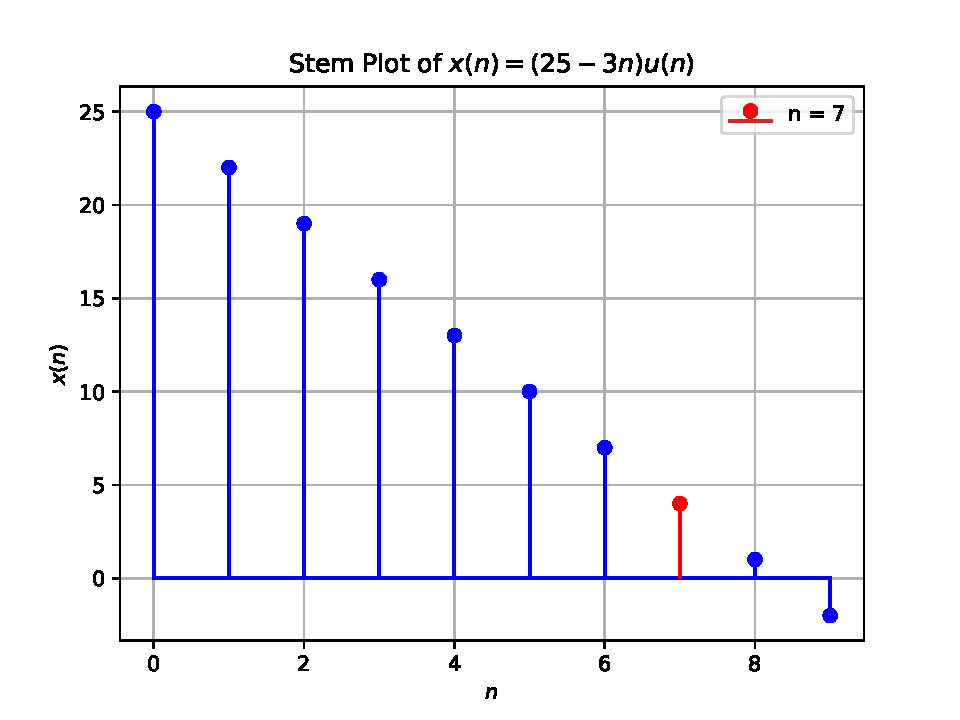
\includegraphics[width=\columnwidth]{figs/stem_plot.pdf}
	
	\label{fig:plot}
\end{figure}
\end{document}

